\documentclass{beamer}

%%% Dichiarazione dei pacchetti standard.
\usepackage[italian]{babel}
\usepackage[utf8x]{inputenc}
\usepackage{graphicx}
\usepackage{natbib}
\usepackage{verbatim}
\hypersetup{pdfsubject={Synthesis of conjugated polymers and quantum dots for photovoltaics applications},pdfkeywords={polythiophene, CdSe, ligand, surface, interfaces, bulk heterojunction, phosphonic acid ligand, Sonogashira, nanocrystals, excitons}} 


%%% Personalizzazione del layout---articolata su cinque livelli.
\usetheme{Warsaw}        % layout complessivo. 
\useinnertheme{default} % layout interno.
\useoutertheme{default} % layout esterno.
\usecolortheme{wolverine} % schema di colori.
\usefonttheme{default}  % schema dei font.
% Inutile dire che se volete tutti i default, potete risparmiarvi gli ultimi
% quattro comandi. 
\setbeamertemplate{headline}[default]
%%% Titolo e autore.


\title{Sintesi controllata di quantum dots stabilizzati da polimeri coniugati funzionalizzati}
\subtitle{Sintesi di materiali per il fotovoltaico ibrido organico-inorganico}
\author{Ilario Gelmetti}
\institute{Scuola Normale Superiore di Pisa}
\date{\today}

\newcommand{\dr}{\textrm}
\def\newblock{\hskip .11em plus .33em minus .07em} 
\beamersetuncovermixins{\opaqueness<1>{25}}{\opaqueness<2->{15}}
\AtBeginSection[]{\frame{ \tableofcontents[current,hideothersubsections]}}

\begin{document}




\begin{frame}
  \titlepage
\end{frame}

\title{Sintesi di quantum dots stabilizzati da polimeri coniugati}





\begin{frame}
\setcounter{tocdepth}{1}
\tableofcontents
\end{frame}

\setcounter{tocdepth}{2}

\section{Quantum dots e fotovoltaico}\subsection{Cosa sono e a cosa servono?}
\begin{frame}
  \frametitle{
  Cosa sono e a cosa servono i \emph{quantum dots}?}
\begin{description}
\item [{Quantum dot}] materiale in cui i portatori di carica hanno zero gradi di libertà spaziale\footnote{Definizione data da Mark Reed nel 1986}. Con questo termine ci si riferisce a nanocristalli semiconduttori inorganici. 
\end{description}

\begin{columns}
	\column{0.6\linewidth}
	Alcune delle moltissime applicazioni sono:
	\begin{itemize}\item Sensori molecolari
	\item Tag fluorescenti in biotecnologia
	\item Tag magnetici
	\item \alert{\textbf{Fotovoltaico}}
\end{itemize}
\column{0.4\linewidth}\begin{figure}
\includegraphics[scale=0.25]{immagini/NPs_come_sensori.png}\caption{Sensori molecolari \tiny{immagine tratta da \emph{Nanoparticles: Scaffolds for Molecular Recognition} - U. Drechsler, B. Erdogan e V. Rotello}}
\end{figure}\end{columns}\end{frame}



  \subsection{Requisiti del fotovoltaico}
    \begin{frame}
      \frametitle{Requisiti del fotovoltaico}
      In una cella fotovoltaica le funzioni minime che il componente assorbente deve svolgere sono:
      \begin{columns}
	\column{0.3\linewidth}
	\begin{itemize}
	  \item Assorbimento della luce e fotogenerazione di eccitoni
	  \item Trasporto degli eccitoni
	  \item Separazione delle cariche
	  \item Trasporto delle cariche
	\end{itemize}
	\column{0.7\linewidth}
	\begin{figure}
	 \includegraphics[scale=0.25]{immagini/livelli.png}\caption{Schema dei livelli energetici di una cella fotovoltaica. \tiny{immagine da \citep{fv-all}}}
	\end{figure}

      \end{columns}
    \end{frame}

  \subsection{Assorbimento e fotogenerazione di eccitoni}
    \begin{frame}
      \frametitle{
      Assorbimento e fotogenerazione di eccitoni}
	L'assorbimento della luce può avvenire
	\begin{itemize}
	  \item da parte del donatore di elettroni (nel nostro caso un polimero, perciò tra HOMO e LUMO),
	  \item da parte dell'accettore (nel nostro caso nanoparticelle semiconduttrici, perciò tra la banda di valenza e la banda di conduzione),
	  \item da parte di un cromoforo inserito appositamente nel sistema.
	\end{itemize}
	Si stima che solo il 10\% delle fotoeccitazioni produca cariche libere \citep{fv-pcbm}, nella maggior parte degli eventi si ha formazione di \alert{eccitoni}\footnote{Eccitone: quasiparticella che descrive lo stato eccitato di un solido. In un semiconduttore, può essere visto come uno stato legato di un elettrone e di una lacuna.}.
    \end{frame}
  \subsection{Separazione delle cariche}

    \begin{frame}
      \frametitle{
      Separazione delle cariche}
      \begin{columns}
	\column{0.6\linewidth}
	\begin{itemize}
	  \uncover<1->{\item Gli eccitoni prodotti hanno una lunghezza di propagazione di circa 10-20 nm \citep{fv-eccit}. }
	  \uncover<2->{\item Per essere spezzati in lacuna ed elettrone devono raggiungere una zona di forte campo elettrico: \alert{un'interfaccia}.}
	  \uncover<3->{\item Dai due punti precedenti segue la necessità di una grande superficie di interfaccia distribuita in tutto il materiale: il \emph{bulk heterojunction}.}
	\end{itemize}
	\column{0.6\linewidth}
	\begin{figure}
	 \uncover<1->{\includegraphics[scale=0.25]{immagini/bilayer-eccitoni.png}\caption{Struttura \emph{bilayer}}}
	\end{figure}\vskip -10pt
	\begin{figure}
	 \uncover<4->{\includegraphics[scale=0.3]{immagini/bulk-heterojunction-eccitoni.png}\caption{Struttura \emph{bulk heterojunction}}}
	\end{figure}
      \end{columns}
    \end{frame}
  \subsection{Trasporto delle cariche}
    \begin{frame}
      \frametitle{
      Trasporto delle cariche}
	\begin{itemize}
	  \item Il trasporto delle cariche è indotto dal potenziale dell'anodo e del catodo esterni.
	  \item Si utilizzano materiali diversi per il trasporto di elettroni e di lacune per \alert{minimizzare la ricombinazione} di questi.
	\end{itemize}\pause
	Le coppie di materiali utilizzati solitamente sono:
	\begin{itemize}
	 \item \alert{Polimero} trasportatore di cariche - \alert{polimero} trasportatore di lacune
	 \item \alert{Polimero} trasportatore di lacune - \alert{nanoparticella} (organica o inorganica) trasportatore di cariche
	\end{itemize}
    \end{frame}
  \subsection{Struttura}
    \begin{frame}
      \frametitle{
      Struttura}
      \begin{columns}
	\column{0.7\linewidth}
	\begin{block}{Perché polimero - nanoparticella?}
	In questa presentazione si prediligeranno sistemi polimero - nanoparticella. Questi sistemi hanno mostrato efficienze maggiori degli altri presentati. 
      \end{block}\pause

	L'architettura del \emph{bulk heterojunction} può essere:
	  \begin{itemize}\pause
	   \item Interconnesse molto aggregate,
	    \item Interconnesse poco aggregate,
	    \item Aggregate in maniera allineata.
	  \end{itemize}
	\column{0.3\linewidth}
	 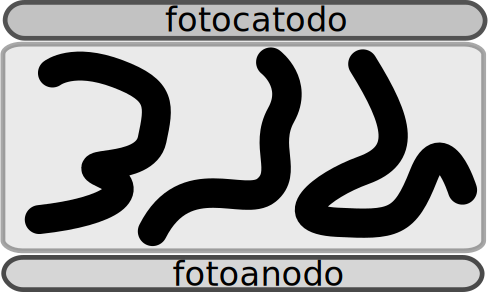
\includegraphics[scale=0.18]{immagini/interconnessi_molto_aggregati.png}\\\vskip 10pt
	  \includegraphics[scale=0.18]{immagini/interconnessi_poco_aggregati.png}\\\vskip 10pt
	 \includegraphics[scale=0.185]{immagini/aggregati_allineati.png}
      \end{columns}
    \end{frame}


\section{Caratteristiche dei materiali}\subsection{Nanoparticelle}

    \begin{frame}
      \frametitle{
      Nanoparticelle}
      Le nanoparticelle si dividono in:
      \begin{columns}
	\column{0.48\linewidth}
	  \begin{itemize}
	    \item organiche
	    \item inorganiche
	  \end{itemize}\pause
	  \begin{block}{Perché inorganiche?}
	  In questa presentazione si prediligeranno nanoparticelle inorganiche. Quest'ultime hanno una \alert{mobilità elettronica} maggiore dei fullereni funzionalizzati \citep{fv-CdSe-OA}. Inoltre hanno alti coefficienti di assorbimento e variandone la dimensione si può variare il \emph{band gap}. 
	  \end{block}\pause
	\column{0.52\linewidth}
      \begin{block}{Perché CdSe?}
	In questa presentazione si prediligeranno nanosfere di CdSe. Per il CdSe sono state riportate in letteratura rese\footnote{resa PCE: \emph{power conversion efficency}} più alte, inoltre il CdSe può essere preparato in nanofili e ramificato. Inoltre i livelli energetici del CdSe sono adatti ad essere utilizzati con molti polimeri conduttori.
      \end{block}
      \end{columns}   
    \end{frame}


  \subsection{Polimeri conduttori}
    \begin{frame}
      \frametitle{ 
 Polimeri conduttori}
      \begin{columns}
	\column{0.55\linewidth}
	I polimeri conduttori impiegati come trasportatori di lacune sono polimeri con una estesa conugazione ed hanno inoltre la funzione di assorbire la luce.
	\begin{itemize}
	   \uncover<2->{\item La separazione HOMO-LUMO dipende dalla lunghezza della coniugazione che, nel caso di buona planarità, raggiunge un massimo di 20 unità,}
	   \uncover<3->{\item le catene laterali non coniugate sono necessarie per dare la plasticità al polimero ma possono impedirne la planarità.}
	\end{itemize}
	\column{0.6\linewidth}\vskip -15pt
	\begin{figure}
	 \uncover<1->{\includegraphics[scale=0.33]{immagini/polimericonduttori.png}\caption{\tiny{immagine da \citet{fv-all}}}}
	\end{figure}
      \end{columns}
    \end{frame}

  
  \subsection{Politiofene}
    \begin{frame}
      \frametitle{ 
 Politiofene}
      \begin{block}{Perché politiofene?}
	In questa presentazione si prediligerà il politiofene come polimero conduttore. A differenza di altri polimeri conduttori il politiofene può esser reso plastico e solubile con delle catene laterali alifatiche. 
      \end{block}
      \begin{columns}
	\column{0.7\linewidth}
	\begin{itemize}
	  \item Lunghezza di coniugazione di 20 unità \citep{pol-pti-lunghezza}.
	  \item La catena laterale più studiata e che verrà utilizzata è l'esile: \emph{poli(3-esiltiofene) P3HT}. 
	  \uncover<3->{\item Per minimizzare la repulsione sterica tra le catene laterali e preservare la planarità il polimero deve essere regioregolare \emph{head-tail-head-tail}.}
	\end{itemize}
	\column{0.3\linewidth}
	\begin{figure}
	    \uncover<3->{\includegraphics[scale=0.45]{immagini/hthttthh.png}\caption{Politiofene sostituito \tiny{immagine da Wikimedia}}}
	\end{figure}

      \end{columns}
    \end{frame}

    \begin{frame}
      \frametitle{ 
 Politiofene}
{\small Si è scelto di rendere il P3HT legante per i QD:
      \begin{columns}
	\column{0.9\linewidth} 
	\begin{itemize}
	   \item catene laterali leganti,
	   \item polimero a blocchi con blocchi leganti,
	   \item entrambe le terminazioni leganti,
	   \item singola terminazione legante.
	  \end{itemize}
	  \begin{block}{Perché legante?}
	   \uncover<2->{ In questa presentazione si prediligeranno politiofeni resi leganti. In questo modo si limita la separazione delle fasi polimero-nanoparticella durante l'evaporazione del solvente.}
	  \end{block}
	  \begin{block}{Perché monofunzionalizzato?}
	    \uncover<3->{In questa presentazione si prediligerà la singola terminazione legante. In questo modo si \alert{evita la formazione di geli reticolati non plastici}. È necessaria la sintesi di un polimero terminato asimmetricamente. }
	  \end{block}
	\column{0.2\linewidth}\vskip -10pt
	\begin{figure}
	   \uncover<1->{ 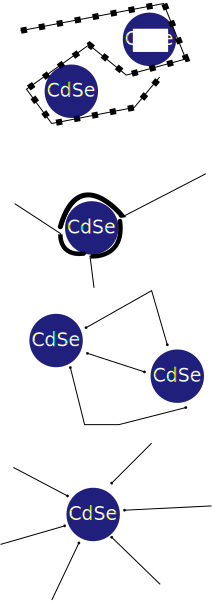
\includegraphics[scale=0.3]{immagini/leganti.png}}
	\end{figure}

      \end{columns}}
    \end{frame}


  \subsection{Schema del sistema oggetto di studio}
    \begin{frame}
      \frametitle{ 
 Schema del sistema oggetto di studio}
	La \textcolor{orange}{composizione} del sistema oggetto di studio è:
	\begin{itemize}
	  \item Quantum dots: nanosfere di CdSe $\phi = 5 - 10 nm$
	  \item Polimero: P3HT poli(3-esiltiofene) monoterminato con gruppo contenente un acido fosfonico
	\end{itemize}\pause
	L'\textcolor{orange}{architettura} del sistema oggetto di studio è un \emph{bulk heterojunction} ossia una dispersione bicontinua.
	\pause Il \textcolor{orange}{processo} di sintesi utilizzato è il seguente:
	\begin{enumerate}
	 \item sintesi di P3HT regioregolare ht-ht terminato asimmetricamente,
	 \item modifica di una terminazione per ottenere un legante acido fosfonico,
	 \item sintesi di nanosfere di CdSe in micella inversa,
	 \item scambio dei leganti presenti sulla superficie delle nanosfere con il nuovo polimero funzionalizzato legante.
	\end{enumerate}
    \end{frame}

\section{Sintesi dei materiali}\subsection{Nanoparticelle}
    \begin{frame}
      \frametitle{ 
 Nanoparticelle}
	Il metodo più semplice, economico e diffuso per produrre nanosfere è la sintesi in micelle inverse.
      \begin{columns}
	\column{0.6\linewidth}
	Alcune delle molte\citep{qd-CdSe-Cd}\citep{fv-CdSe-OA}\citep{lig-CdSe-P}\citep{lig-p3ht-CdSe-end}, sorgenti di Cd e di Se sono:
	\begin{itemize}
	  \item Me$_2$Cd + TOPSe (seleniuro di triottilfosfina) \citep{qd-CdSe-Cd},
	  \item CdCl$_2$ + NaHSe + TOP \citep{qd-CdSe-CdCl2}.
	\end{itemize}
	\column{0.4\linewidth}\pause
	  \begin{block}{Perché CdCl$_2$ + NaHSe?}
	    In questa presentazione si prediligerà la sintesi da CdCl$_2$ e NaHSe. Il Me$_2$Cd è volatile, tossico ed esplosivo. La sintesi da CdCl$_2$ e NaHSe è più sicura, meno costosa, utilizza reagenti non troppo tossici ed è veloce.
	  \end{block}
	\end{columns}\vskip 10pt
    \pause Per \alert{impedire l'aggregazione} delle nanosfere si utilizza il legante trioctilfosfina ossido TOPO.
    \end{frame}


    
    
    
  \subsection{Politiofene regioregolare}
    \begin{frame}
      \frametitle{
Politiofene regioregolare}

	La polimerizzazione per metatesi Grignard adeguatamente catalizzata può realizzare P3HT poli(3-esiltiofene) regioregolare.
	 
	
	\begin{itemize}
	  \item Partendo da 2,5-dibromotiofene si produce il monomero reattivo. La regioselettività di questa reazione è elevata.
	  \item Per avere una alta regioregolarità \emph{ht-ht} nel metodo GRIM \emph{Grignard metathesis} si usa cloruro di [1,2-Bis(difenilfosfino)propano]nickel Ni(DPPP)Cl$_2$ \citep{pol-p3ht-end}.
	\end{itemize}
	\begin{figure}
	  \includegraphics[scale=0.35]{immagini/tiofene+mg.png}\caption{Preparazione del monomero secondo il metodo GRIM.}
	\end{figure}
    \end{frame}


  \subsection{Politiofene terminato asimmetricamente}
    \frame[plain]{
	Alcuni reagenti di Grignard aggiunti al P3HT Br/Br formato lo terminano solo ad una terminazione, altri lo terminano in entrambe.
	\vskip -10pt
	\begin{figure}
	  \includegraphics[scale=0.085]{immagini/pol-endcapping2.png} \\ \tiny{Ipotesi di meccanismo di reazione. Immagine tratta da \citet{pol-p3ht-end}}
	\end{figure}\vskip -10pt
	Per avere il polimero prevalentemente monoterminato si può utilizzare \includegraphics[scale=0.38]{immagini/grignard-monocap.png}
}


  \subsection{Modificazione di una terminazione del politiofene}
    \begin{frame}
      \frametitle{Modificazione di una terminazione del politiofene}

      \begin{block}{Perché \textbf{R'} = allile?}
	In questa presentazione si prediligerà la sintesi di P3HT terminato allile/Br. Questa terminazione è risultata meno problematica di quella etinilica presentando rese maggiori.
      \end{block}
\pause
	Una possibile via per rendere legante il P3HT è modificare il Br terminale con il \emph{coupling} di Sonogashira:
	\begin{figure} 
	\includegraphics[scale=0.40]{immagini/p3ht+legantegenerico.png}
	\end{figure}
    \end{frame}


  \subsection{Scambio dei leganti}
    \begin{frame}
      \frametitle{
Scambio dei leganti}
      Si è deciso di sostituire il TOPO trioctilfosfina ossido passivante la superficie dei \emph{quantum dots} in modo da ottenere il polimero conduttore direttamente legato. 
 \pause     \\Una \alert{\bf{indicativa} }scala di affinità decrescente può essere così estrapolata dalla letteratura\citep{lig-CdSe-caratt} \citep{lig-CdSe-P} \citep{fv-CdSe-OA}:
      \begin{columns}
	\column{0.5\linewidth}
	\begin{enumerate}
	 \item acidi carbossilici,
	 \item ammine primarie,
	 \item mercaptani,
	 \item priridine 4-sostituite,
	 \item monoalchil fosfonati,
	 \item triottilfosfina ossido,
	 \item dialchil fosfinati,
	\end{enumerate}
	\column{0.5\linewidth}
	\begin{block}{Perché monoterminato fosfonico?}
	    Si prediligeranno leganti monodentati acidi fosfonici. Si modifica una sola terminazione per evitare la formazione di geli reticolati.
	\end{block}
      \end{columns}
    \end{frame}

  



\section{Una possibile via}\subsection{Sintesi Politiofene tramite metatesi Grignard}
    \begin{frame}
      \frametitle{Una possibile via}\framesubtitle{Sintesi Politiofene tramite metatesi Grignard}
      Una possibile via sintetica del P3HT regioregolare \emph{ht-ht} terminato Br/allile è riportata da \citet{lig-p3ht-CdSe-end}:

	\begin{figure}
	  \includegraphics[scale=0.27]{immagini/grim+end.png}
	\end{figure}
	Le tecniche di caratterizzazione che verranno utilizzate sono: $^1$H-NMR, FTIR, UV-Vis e fluorescenza.

    \end{frame}


  \subsection{Modifica di una terminazione del politiofene}
    \begin{frame}
      \frametitle{Una possibile via}\framesubtitle{Modifica di una terminazione del politiofene}
      Il precursore estere fosfonico viene modificato tramite Sonogashira coupling in modo da contenere un triplo legame che con un ulteriore coupling si lega con l'altra terminazione al P3HT.

\citep{sonog-rev}
	\begin{figure} 
	\includegraphics[scale=0.34]{immagini/sintesilegantepro.png}
	\end{figure}
	\begin{figure} 
	\includegraphics[scale=0.34]{immagini/p3ht+legante.png}
	\end{figure}\pause
	Le tecniche di caratterizzazione che verranno utilizzate sono: $^1$H-NMR, FTIR, DSC (\emph{differential scanning calorimetry}) e TGA (\emph{thermogravimetric analysis}).
    \end{frame}


  \subsection{Sintesi dei quantum dots}
    \begin{frame}
      \frametitle{Una possibile via}\framesubtitle{Sintesi dei quantum dots}
      Una procedura economica e che utilizza reagenti non troppo tossici è quella messa a punto da \citet{qd-CdSe-CdCl2}:

 $$ 4\dr{NaBH}_4 + 2\dr{Se} + 7\dr{H}_2\dr{O} \longrightarrow 2\dr{NaHSe} + \dr{Na}_2\dr{B}_4\dr{O}_7 + 14\dr{H}_2 $$
    $$\dr{NaHSe} + \dr{CdCl}_2 \longrightarrow \dr{CdSe} + \dr{NaCl + HCl} $$
    Dopo alcuni passaggi si ottengono le nanosfere passivate da TOPO e si precipitano con metanolo.\\ \vskip 15pt \pause
	Le tecniche di caratterizzazione che verranno utilizzate sono: UV-Vis, fluorescenza, DLS (\emph{dynamic light scattering}).

    \end{frame}


  \subsection{Scambio dei leganti}
    \begin{frame}
      \frametitle{Una possibile via}\framesubtitle{Scambio dei leganti}
      Una possibile procedura per lo scambio dei leganti è quella seguita da \citet{qd-CdSe-caratt}.
      \begin{figure}
	\includegraphics[scale=0.27]{immagini/scambio-leganti.png}
      \end{figure}\pause
      	Le tecniche di caratterizzazione che verranno utilizzate sono: FTIR, TGA (\emph{thermogravimetric analysis}), DLS (\emph{dynamic light scattering}).

    \end{frame}






\tiny{
\bibliographystyle{plainnat}
\bibliography{modulo_primo.bib}
}

    \begin{frame}
     \center{\Huge{Fine.}\vskip 30pt
     \tiny{Presentazione realizzata con
     \\\LaTeX \\ \textsc{beamer}
     \\Debian Squeeze}}


    \end{frame}



\end{document}
